\section{Study Settings}
\label{method}

The main goal of this research is to investigate the impact of atoms of confusion in JavaScript code comprehension. As such, in this paper we answer the following research questions: 

\begin{enumerate}[(RQ1)]
    \item Do JavaScript developers identify atoms of confusion as contributing to program misunderstanding? 
    \item What is the impact of atoms of confusion on the comprehension of JavaScript code? 
    \item What are the particular JavaScript idioms and language constructs that might cause source code misunderstanding?
    \item What is the frequency of occurrence of atoms of confusion in practice (i.e., in open-source JavaScript projects)?
\end{enumerate}

 
Answering these research questions has several implications. For instance, we can either generalize or refute the perceptions about atoms of confusion already discussed in the literature (goal of research questions (RQ1) and (RQ2)). In addition, answers to the third and fourth questions allow us to enrich existing catalogs about atoms of confusion and discuss how often they occur in practice. Our motivation to detect the presence and impact of atoms of confusion is also motivated by the possibility of laying the foundations for the implementation of libraries that can automatically transform code into its cleaner versions---though we postpone these results to a future research work. This might lead to a new catalog of refactoring for removing atoms of confusion.  To answer these research questions we conduct a mixed-methods study, including a survey, a set of interviews, and an effort of mining JavaScript software repositories.  


 \subsection{First Study: Survey}\label{sec:survey-settings}\castor{Eu mudaria os títulos desta sub-seção e das duas próximas para "First study: Survey", "Second study: Mining open source repositories", etc. Vale a pena manter "First study", etc.?}
% \subsubsection{The Atoms Considered In This Work}

In the first study, our goal was to collect evidence to answer two specific questions: 
\begin{itemize}
    \item \emph{Do code snippets that contain atoms of confusion produce a higher misunderstanding rate when programmers try to predict their outcome?}
    \item \emph{Do code snippets with atoms of confusion require programmers to take longer to predict their output?}
\end{itemize}

To address these questions we conducted a survey to assess the impact of atoms of confusion on understanding JavaScript code. Since JavaScript and C have some constructs in common (Section~\ref{sec:aoc}), we first selected a set of atoms of confusion for the \clang language~\cite{DBLP:conf/sigsoft/GopsteinIYDZYC17} that may also exist in JavaScript programs. {\color{red}In addition, we consider a particular atom that is exclusive to JavaScript in this first study}. Appendix~\ref{sec:appendix-atoms} summarizes all atoms we consider in our research. 

\subsubsection{Survey design} 

The design of our first study aims to block two variables (developer experience and the code snippets) and considers two treatments: the presence or absence of 
atoms of confusion within the code snippets. 
To achieve such a design goal, controlling the effect of experience and individual code snippets, we resorted to the \textit{Latin Square Design} \cite{Hunter-Experimenters}. Using this design we create a 2 x 2 matrix in which each row represents a subject and each column indicates the set of code snippets. The design of each square (a replica) is such that no treatment is repeated in the same row or column. For example, if a given subject (P1) is asked to predict the output of code snippets that contain atom candidates \texttt{\{1,2,3,4,5\}}, then, when answering questions about non-confusing code snippets, they will only be presented with non-confusing versions of atom candidates \texttt{\{6,7,8,9,10\}}. Furthermore, a given subject (P2), which constitutes the second row of our example square, will be asked questions about the non-confusing versions of \texttt{\{1,2,3,4,5\}}, and will answer questions about confusing snippets of \texttt{\{6,7,8,9,10\}}. By doing that, we guarantee that all of our 20 snippets are contained within each square, and that each configuration occurs only once within a square. Figure \ref{fig:latinsquare} offers a visual representation of the concept.

  \begin{figure}[htb!]
      \noindent
      \centering
      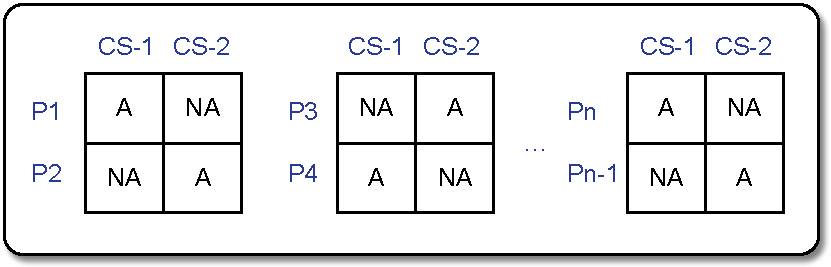
\includegraphics[scale=.50]{images/latin-square.pdf}
      \caption{Latin square design. Each ``square'' corresponds to 
      a replica in our study. Each replica comprises two students (square rows) 
      and two sets of code snippets (CS-1 and CS-2). We randomly apply the 
      treatments (atom or non-atom code) to the cells of the squares.} 
      \label{fig:latinsquare}
  \end{figure}


Having selected 10 atoms in our first study, we wrote small pieces of code that contained each atom. We also wrote their equivalent snippet without the confusing idioms and constructs, leading to a total of 20 code snippets. In order to reduce the cognitive effort, we decided that each subject would be asked to predict the output of a subset of 10 listings, wherein each subset contained 5 blocks that contained atoms of confusion, whilst the remaining 5 had the atoms removed. The order in which the questions were presented was randomized. By doing this, we were seeking to minimize the chances of subjects being aware that the current listing they were analyzing contained (or not) atoms of confusion.
That is, each respondent of the survey should indicate what would be the outcomes of the code snippets, some of them having atoms of confusion (while other code snippets did not). 
We measured answer correctness and total time each participant needed to answer reach question of their survey. 

\subsubsection{Survey Instrument} 

We implemented our survey as a web application. As part of this 
effort, we carried out an informal pilot whose main objectives were: to spot bugs in the application and in the data collection mechanism; to gain feedback from respondents about the user experience of the application; and to formulate an estimate about how long answering the survey would, on average, take. Fellow undergraduate students, professional colleagues, and friends took the pilot survey. Some users reported layout defects, and many reported that the landing page did not explain the survey well enough. We also spotted minor issues with our routines to create and populate the Latin Squares. 

We organized the survey in {\color{red}three} sections. The first section aims to characterize the subjects, asking for their age, education level, and programming experience. We also included a check button, whose checking meant users agreed that all collected data would be used solely for research purposes. In the second section, we presented to the participants a small set of instructions, where we explained how the survey worked and asked them to dedicate their attention to it. We stressed to participants the importance of not using any aids during the survey, such as online or console interpreters. For each question page, we kept track of whether or not the subjects switched windows. 

The next section of the survey presented a sequence of 10 questions, each containing a code snippet. For each question, there was a text box where the answer should be written. There was also an ``I do not know'' button, which, when clicked, led the subject to the next question. In our setting, ``I do not know'' was treated as a wrong answer. The code snippets were presented as images copied from a text editor, so as to demotivate respondents from resorting to external resources by copying and pasting the code into an interpreter. Upon submitting their answer for a particular question, the subject was automatically led to a similar page, containing another snippet.
    
We decided not to provide feedback about the time students took to answer each question. Nor did we tell them whether their answers were correct or not. Our main concern was to avoid introducing bias for future respondents. Since we posted the survey in a social media platform, if we gave respondents instant feedback, they might post comments on particular atoms, therefore interfering with future participants' thought process.

% \rb{nao acho esse paragrafo necessario} 
% \adriano{o de baixo ne? eu tambem acho}

% As we mentioned before, we first wrote the code listings in a text editor, and took pictures of it. In the case of an atom of confusion that was exclusive to JavaScript, which we called \textit{Automatic Semicolon Insertion} (see Appendix~\ref{sec:appendix-atoms}), it was necessary to remove the syntax highlighter. Even though semicolons at the end of statements are optional to programmers in JavaScript, the interpreter automatically inserts them into the code. Our text editor was incorrectly highlighting a line break after a return statement, even thought it was valid JavaScript syntax. We had thus to turn the highlighter off to take the picture of this atom. 

\subsubsection{Survey audience}

\diego{Esses detalhes são possíveis candidatos para remoção, se precisarmos de espaço}
{\color{blue}We invited developers to answer our survey by sending invitations to communities of JavaScript programmers on the Internet. Our initial plan was to try to engage contributors for two major JavaScript projects, namely Node.js and NPM. None of the projects, though, offered a direct way to interact with the community, such as an online discussion forums or mailing list. We would be required to first make contact with the projects' leaders, and only then would we have a chance to approach potential respondents. Due to time constraints, we decided to look for respondents elsewhere.}
We then posted the survey on Reddit.\footnote{Reddit is a North American online discussion platform. Its discussion threads, often called subreddits, are sorted by subject. For our research, we posted information and links to the survey in two JavaScript subreddits.}. We explained our research purposes, and asked developers of any level of expertise to take the survey. To incentivize serious engagement, we proposed to raffle \$50 gift cards on Amazon products at the end of the survey. Within twelve hours we collected more than 150 answers, populating more than 70 replicas of the Latin Squares. We were able to collect significant data on time taken and discrepancies in answer correctness between confusing and non-confusing versions of the snippets. 
    
\rb{acho que podemos mover esse proximo paragrafo para a secao de resultados, ou de ameacas}
\adriano{acho que pode ir para resultados. nao considero uma ameaca pois eu e o Caio tratamos manualmente as entradas a serem removidas e garantimos a integridade dos latin squares}

Inconsistencies may arise when each square is being built. The main source of inconsistency we faced was when a user quit in the middle of the survey. When this happened, his row in the square was left incomplete. We considered all squares which contained incomplete rows to be invalid, and discarded them. Since we had a large enough number of samples, the squares we had to discard did not impact our results.
    
    
% \subsubsection{Pilot Survey}    

% To validate the web application we developed to conduct the survey, we ran an informal pilot survey whose main objectives were:
%     \begin{itemize}
%         \item To spot bugs in the application and in the data collection mechanism;
%         \item To gain feedback from respondents about the user experience of the application;
%         \item To formulate an estimate about how long the survey would, on average, take.
%     \end{itemize}
    
% We had fellow undergraduate students, work colleagues and friends take the pilot survey. We discovered that the aspect that needed most improvement was the user experience. Some users reported layout defects, and many reported that the landing page did not explain the survey well enough. We also spotted minor issues with our routines to create and populate the Latin Squares. After performing all the necessary changes, we were ready to conduct another experiment.

\rb{Comentei o survey com alunos}

% \subsubsection{A Survey With Undergraduate Students}
%     Our second attempt was due to courtesy of a professor of our department. During the semester of the writing of this text, he was lecturing a Data Structures course, which is usually taken during the second semester of the undergraduate course. The professor agreed to take the students to a laboratory during one of his classes, and all the students who attended that day took the survey.
    
%     No issues were reported with the web application, and all answers were appropriately collected. This time, all the Latin Squares were being populated correctly, making the data we collected eligible for use in the final analysis. However, we opted to dispose of all the data we gathered in this occasion. What motivated this decision were the two following aspects:
%     \begin{enumerate}
%         \item The students were not focusing hard enough. Most students were not very serious about the survey. While we watched them answer the questions, we could see many students peeking at each other's screens. We could also clearly see students not taking nearly enough time to reason about the code, and answering the questions without giving it proper thought.
%         \item We needed a more diverse spectrum of respondents. In the beginning of our research, we established that we would need at least 25 Latin Squares in order to be able to have significant results. By conducting this survey, we were able to populate 11 Latin Squares. Compounded by the problem reported above, we were concerned that our spectrum of respondents might end up skewed towards undergraduate students with little or no JavaScript programming experience.
%     \end{enumerate}
    
%     These two facts led us to conclude we needed to conduct a survey in which partakers engaged voluntarily, whilst also having an incentive to think hard enough about the problems they faced. To address these points, we prepared our final setting.
    
\subsection{Second Study: Mining Software Repositories}

To understand how often atoms of confusion appear in real settings, and thus answer our fourth research question (\emph{What is the frequency of occurrence of atoms of confusion in practice?}), we mined a set of GitHub open source repositories. To this end, we first collected the most popular GitHub repositories that are primarily written is JavaScript. We measured popularity using the project's stargazers, and selected only projects with stargazers\_count > 100. This metric, available on  GitHub API, represents the number of stars a project received from users of the platform. The same metric has been used in a number of previous studies as a proxy to estimate project's popularity~\cite{gyimesi2019bugsjs}.

After filtering out JavaScript project candidates, in the second step we built a curate dataset comprising the top 100 most popular repositories. Examples of projects in this dataset include \textsc{React}, \textsc{Node JS}, and \textsc{AngularJS}. Table~\ref{tab:projects-statistics} presents some statistics about the projects we consider in our research. The size of the projects range from small ones (883 liens of code) to complex systems with more than 10 MLOC. All projects in our dataset have at least \num{1161} forks and \num{23643} stars. We automated all the steps to filter, clone, and collect the statistics from the repositories using Python scripts.

In the third step we mined atoms of confusion from the repositories in our curate dataset. We written source code queries usng the CodeQL language~\cite{moor:gttse2007}, in order to filter the atoms of confusion. CodeQL is an object-oriented variant of the Datalog language~\cite{rodriguez2020efficient}, and currently supports researchers and practitioners to query the source code of systems written in different languages (such as Java and JavaScript). 
We also automate the process of running the queries and exporting the results to a format that simplifies our analysis and the reproduction of this study. In the final step we carry out basic descriptive statistics, in order to understand how often the atoms of confusion appear in practice. 

\begin{table*}[ht]
 \centering
 \begin{tabular}{rrrrrrr}
   \hline
             & Min. & 1st Qu. & Median & Mean & 3rd Qu. & Max. \\ \hline
 Lines of Code           & \num{883}  & \num{14939} & \num{39520} & \num{281088.46} & \num{145990.75} & \num{10149685} \\
 Num. of Contributors    & \num{6}   & \num{121} & \num{243} & \num{431.82} & \num{436.75} & \num{4042} \\
 Num. of Forks           & \num{1161}   & \num{3365} & \num{5711} & \num{8201.96} & \num{8438.25} & \num{68826} \\
 Num. of Stars        & \num{23643} & \num{27542.25} & \num{35687.5} & \num{45284.86} & \num{47963.25} & \num{310725} \\
    \hline
 \end{tabular}
 \caption{Some descriptive statistics about the projects used in the study}
 \label{tab:projects-statistics} 
 \end{table*}
 
\subsection{Third Study: Interviews with Practitioners}

To complement our initial survey, we performed semi-structured interviews with professional JavaScript developers, aiming to identify their perceptions regarding code snippets containing atoms of confusion. We also asked each participant if they knew of any other JavaScript-specific construct that they regarded as confusing. In this section we details the protocol we followed to conduct the interviews, and we also describe how their results were analysed.

% Nós realizamos entrevistas semi-estruturas com o objetivo de identificar a percepção dos desenvolvedores com experiência em JavaScript sobre algumas questões relacionadas à compreensão de código em JavaScript. Assim, nesta Seção nós descrevemos os procedimentos adotados para selecionar os participantes para as entrevistas e detalhamos como as entrevistas foram conduzidas. Além disso, detalhamos como os resultados das entrevistas foram analisados.

\subsubsection{Participants Selection}: The participants of the interviews were invited personally by the authors, and the pool of potential participants was based on our network of contacts. Our main criterion of selection was that all participants had to be working professionally with JavaScript. We invited a total of 17 developers, and 15 of these agreed to participate, and throughout a two week period, we conducted all the interviews.

% Os participantes das entrevistas foram selecionados a partir da nossa rede de contatos. Nós convidamos 17 pessoas e 2 não responderam ao nosso convite para participar das entrevistas. Durante 2 semanas, nós entrevistamos 15 desenvolvedores. Iniciamente nós conduzimos duas entrevistas como piloto. Após o piloto com dois desenvolvedores com mais de 03 anos de experiência, nós adicionamos uma nova pergunta na entrevista: Você conhece alguma construção em JavaScript que leve a um mal entendimento do código? Ao finalizar as entrevistas, nós perguntamos ao desenvolvedor se ele conhecia algum outro desenvolvedor com experiência em JavaScript que pudesse nos indicar para participar das entrevistas. Nós entrevistamos 02 desenvolvedores a partir da indicação dos entrevistados. A Tabela \ref{pinterview} apresenta o perfil dos 15 participantes das entrevistas.

\subsubsection{Interview Process}

We conducted semi-structured interviews using a web conferencing software. All the interviews were recorded with the consent of participants. On average, the interviews lasted 26.29 minutes, with the shortest one lasting 14.59 minutes, and the longest one 43.06 minutes. The main goal of the interviews was to have developers assess in real time whether two versions of code with the same behavior differed in readability, and, if so, which version they regarded as the easier one to understand. The interviews were conducted by two of the authors of this text, and a third one listened to all the recordings to cross-validate the collected data.

% Nós conduzimos entrevistas semi-estruturadas utilizando um software de conferência de audio/video. Todas as entrevistas foram gravadas com o consenso dos entrevistados. As entrevistas tiveram uma duração de aproximadamente 26.29 minutos. A entrevista com menor duração foi de 14.59 minutos e de maior duração foi de 43.06 minutos. O objetivo ao realizar as entrevistas era identificar quais as construções em JavaScript podem corresponder a confusões de código. As entrevistas foram realizadas por dois dos autores deste artigo.

The interviews had three main parts. In the first one, we asked the developers the following demographic information: name, email, gender, level of education, current job position, JavaScript experience and other programming languages they have worked with. Table \ref{pinterview} presents the profile of each participant.

\begin{table*}[htb!]
\centering
\begin{tabular}
{|p{0.4cm}|p{0.9cm}|p{2.0cm}|p{7.0cm}|p{1.9cm}|p{3.0cm}|}
\hline
ID & Gender & Level & Role & JS Experience & Other Languages \\ \hline  
P1 & Male & Graduate & Developer at Federal Court of Accounts - TCU Brazil & 9 years & Java, PHP, C, Go  
\\ \hline
P2 & Male & High School & Developer at Luma Health & 3.5 years & Python, Go, Dart, Lua, C++, C\#
\\ \hline
P3 & Male & Graduate & Developer at Superior Labour Court - TST Brazil & 4 years & Java, C
\\ \hline
P4 & Male & Undergraduate & Developer at Brazilian Association of Research and Industrial Innovation - EMBRAPII & 3 years & Python, C, C++, Java, Go
\\ \hline
P5 & Male & Master Student & Developer na Qubo Technology & 3 years & Python, SQL
\\ \hline
P6 & Male & Graduate & Software Architect at Superior Labour Court - TST Brazil & >15 years & Java, PHP, C, Python , Ruby, C\# and R
\\ \hline
P7 & Male & Graduate & Developer na Stefanini & 6 years & C, C++, Java, Assembly, Kotlin
\\ \hline
P8 & Male & PhD & Developer Regional Labour Court - TRT Goiás, Brazil & 2 years & Java, Python
\\ \hline
P9 & Male & Graduate & IT Analyst at Regional Bank of Brasilia - BRB Brazil & 5 years & PHP
\\ \hline
P10 & Male & Master Student & Business Analyst and Developer at National Confederation of Industry - CNI Brazil & 4 years & Java, C\# and Python
\\ \hline
P11 & Male & Master Student & Software Architect at the University of Brasilia's Informatics Centre & 4 years & Java, Erlang, C\#, Cobol
\\ \hline
P12 & Female & Master & Software Engineers at Novatics & 1 year & C
\\ \hline
P13 & Male & Master & Developer at the Military Police of the Federal District - PMDF Brazil & 13 years & Java, PHP
\\ \hline
P14 & Female & Master Student & Developer at Neoway & 3 years & C, Python, Ruby
\\ \hline
P15 & Female &  Graduate & Developer at SICOOB & 2 years & Java, PHP
\\ \hline
\end{tabular}
    \caption{Demographic information of the participants}
    \label{pinterview}
\end{table*}

The second part of the interview was more open, and our aim here was to allow the subjects to describe their JavaScript experience, as well as to allow them to make suggestions about any JavaScript's constructs they regarded as innately confusing, as this would allow us to include their suggestions in future work. The questions asked in this section were:
\begin{itemize}
    \item In general, do you implement new JavaScript components, or do you maintain components developed by other programmers?;
    \item In your opinion, what are the main pros and cons of the language?;
    \item Do you think JavaScript is a language that produces code that is hard to understand?
    \item Do you regard any particular construct of the language as especially confusing?
\end{itemize}

\rb{acho melhor mover os code snippets da entrevista para um apendice online. deixei comentado aqui.}
\adriano{como os snippets sao os mesmos do TCC, a ja temos o apendice, nao poderiamos colocar no apendice B deste texto? posso escrever os snippets no repositorio tambem. deixa-los no apendice pode tornar o paragrafo abaixo mais compreensivel/verificavel.}

In the third part of the interview, participants were shown the 20 code snippets that were used to build the aforementioned Latin Squares. The participants were told both sides of each pair had the same output, and were asked to evaluate which construct was easier to understand. The interviewers restrained themselves from introducing bias into the answers by not explaining that one of the sides of each pair contained the atom under investigation. Subjects were just presented the snippets and allowed to take the necessary time to decide on the most readable snippet.

% As entrevistas foram divididas em três etapas. Na primeira etapa da entrevista nós perguntamos aos desenvolvedores as seguintes informações: Nome; E-mail; Gender; Level; Role; Experience; Quais as outras linguagens de programação ele/ela conhecia. Na segunda etapa da entrevista,  perguntamos aos desenvolvedores: a) No geral você escreve novos componentes em JavaScript, ou você faz manutenção em componentes desenvolvidos por outra pessoa (explique o seu dia-a-dia); b) Na sua opinião, quais são os pontos fortes e fracos da linguagem JavaScript. c) Você acha que a linguagem JavaScript é uma linguagem que leva a um código difícil de ser compreendido? d) Tem alguma construção em JavaScript que você conhece que pode levar a uma dificuldade de entendimento. Na terceira etapa da entrevista nós apresentamos alguns exemplos de trechos de código em JavaScript, contendo os 10 tipos de construção apresentados na Table \ref{tab:atoms} com e sem átomos de confusão (Lado A e Lado B), conforme apresentado na Table \ref{snippets}. Nós perguntamos aos desenvolvedores: 1) Você acha que o código do lado B prejudica de alguma forma a compreensão do código? Os dois códigos apresentados nos dois lados de alguma maneira eram equivalentes. 

% \begin{longtable}
% {| p{.50\linewidth} | p{.50\linewidth} |} 
% % \begin{center}
% \caption*{Code Snippets presented on the interview}
% \label{snippets}
% % \begin{tabular}{ | p{8.2cm} | p{8.2cm} | } \hline
% \hline
% \multicolumn{2}{| c |}{Arithmetic as Logic}  \\ \hline
% Side A  &  Side B \\ \hline
% \begin{lstlisting}[language=JavaScript]
% let array_1 = [1,2,3];
% let array_2 = [2,3,2];
% if(array_1.length - array_2.length){
%   console.log(true);
% }
% else{
%   console.log(false);
% } \end{lstlisting}
% & 
% \begin{lstlisting}[language=JavaScript]
% let array_1 = [1,2,3];
% let array_2 = [2,3,2];
% if(array_1.length != array_2.length){
%   console.log(true);
% }
% else{
%   console.log(false);
% } \end{lstlisting} \\ \hline
% \multicolumn{2}{| c |}{Assignment as value}  \\ \hline
% Side A  &  Side B \\ \hline
% \begin{lstlisting}[language=JavaScript]
% function resetSchedulerState () {
%   let activatedChildren = {length: 10};
%   let index = length = activatedChildren.length = 0;
%   console.log(index);
% }
% resetSchedulerState(); \end{lstlisting}
% & 
% \begin{lstlisting}[language=JavaScript]
% function resetSchedulerState () {
%   let activatedChildren = {length: 10};
%   activatedChildren.length = 0;
%   let length = activatedChildren.length;
%   let index = length;
%   console.log(index);
% }
% resetSchedulerState(); \end{lstlisting} \\ \hline
% %\pagebreak 
% \hline
% \multicolumn{2}{| c |}{Automatic Semicolon Insertion}  \\ \hline
% Side A  &  Side B \\ \hline
% \begin{lstlisting}[language=JavaScript]
% function example(){
%   return
%       10
% }
% if(example() == 10){
%   console.log(true);
% }
% else{
%   console.log(false);
% } \end{lstlisting}
% & 
% \begin{lstlisting}[language=JavaScript]
% function example(){
%   return 10;
% }
% if(example() == 10){
%   console.log(true);
% }
% else{
%   console.log(false);
% } \end{lstlisting} \\ \hline
% \multicolumn{2}{| c |}{Comma Operator}  \\ \hline
% Side A  &  Side B \\ \hline
% \begin{lstlisting}[language=JavaScript]
% let V1 = 5, V2 = 10;
% V1 = (V2 = 1, 2);
% console.log(V1+V2);
% \end{lstlisting}
% & 
% \begin{lstlisting}[language=JavaScript]
% let V1 = 5, V2 = 10;
% V2 = 1;
% V1 = 2;
% console.log(V1+V2);
% \end{lstlisting} \\ \hline
% %\pagebreak
% \hline
% \multicolumn{2}{| c |}{Ternary Operator}  \\ \hline
% Side A  &  Side B \\ \hline
% \begin{lstlisting}[language=JavaScript]
% let config = {size: 3, isActive: false};
% const _config = config.isActive === true ? config : {size: 10};
% console.log(_config.size); \end{lstlisting}
% & 
% \begin{lstlisting}[language=JavaScript]
% let config = {size: 3, isActive: false}
% let _config;
% if(config.isActive === true){
%   _config = config;
% }
% else{
%   _config = {size: 10};
% }
% console.log(_config.size); \end{lstlisting} \\ \hline

% \multicolumn{2}{| c |}{Implicit Predicate}  \\ \hline
% Side A  &  Side B \\ \hline
% \begin{lstlisting}[language=JavaScript]
% let V1 = 10, V2 = 3;
% if (!(V1 % V2)){
%   console.log(true);
% }
% else{
%   console.log(false);
% } \end{lstlisting}
% & 
% \begin{lstlisting}[language=JavaScript]
% let V1 = 1, V2 = 2;
% if ((V2 - V1) == 0){
%   console.log(true);
% }
% else{
%   console.log(false);
% } \end{lstlisting} \\ \hline
% \multicolumn{2}{| c |}{Logic Control Flow}  \\ \hline
% Side A  &  Side B \\ \hline
% \begin{lstlisting}[language=JavaScript]
% let V1 = 3;
% let V2 = 5;
% let V3 = 0;
% while (V1 != V2 && ++V1) {
%   V3++;
% }
% console.log(V1 + V3); \end{lstlisting}
% & 
% \begin{lstlisting}[language=JavaScript]
% let V1 = 1;
% let V2 = 11;
% let V3 = 0;
% while (V1 != V2) {
%   V1++;
%   V3++;
% }
% console.log(V1+V3); \end{lstlisting} \\ \hline
% \multicolumn{2}{| c |}{Omitted Curly Braces \& Indentation}  \\ \hline
% Side A  &  Side B \\ \hline
% \begin{lstlisting}[language=JavaScript]
% let V1 = 1, V2 = 2
% if (V1 > V2)
% V2 = 1
% V1 = 2
% console.log(V2+V1) \end{lstlisting}
% & 
% \begin{lstlisting}[language=JavaScript]
% let V1 = 1, V2 = 2;
% if (V1 > V2) {
%   V2 = 1;
% }
% V1 = 2;
% console.log(V2+V1); \end{lstlisting} \\ \hline
% \multicolumn{2}{| c |}{Post Increment}  \\ \hline
% Side A  &  Side B \\ \hline
% \begin{lstlisting}[language=JavaScript]
% let V1 = 0;
% if (V1++ == 0) {
%   console.log(true);
% }
% else {
%   console.log(false);
% } \end{lstlisting}
% & 
% \begin{lstlisting}[language=JavaScript]
% let V1 = 0;
% if (V1 == 0) {
%   console.log(true);
% }
% else {
%   console.log(false);
% }
% V1 = V1 + 1; \end{lstlisting} \\ \hline
% \multicolumn{2}{| c |}{Pre Increment}  \\ \hline
% Side A  &  Side B \\ \hline
% \begin{lstlisting}[language=JavaScript]
% var index = 1;
% while (++index < 10) {
%   console.log(index);
%   break;
% } \end{lstlisting}
% & 
% \begin{lstlisting}[language=JavaScript]
% var index = 0;
% index = index + 1;
% while (index < 10) {
%   console.log(index);
%   index = index + 1;
%   break;
% } \end{lstlisting} \\ \hline
% % \end{tabular}
% % \end{center}
% % \end{table}
% \end{longtable}

\subsubsection{Interview Analysis}

Nós realizamos a análise das entrevistas em pares. Inicialmente um dos participantes de todas as entrevistas transcreveu os resultados. Posteriormente, um dos autores do trabalho ouviu os áudios das entrevistas e transcreveu os resultados. 

\textcolor{red}{Adriano teria algo mais para adicionar aqui na  análise das entrevistas?}

\todo[inline]{adriano:estou escrevendo uma tabela em que cada linha e um dos atomos, e colunas representam \% preferencia com atomo, \% preferencia sem atomo, \% indiferente. Mas acredito que esta tabela deve estar na section results, certo? O resto das informacoes deste paragrafo eu citei acima no Interview Process, entao acho que podemos abolir esta section. -- Edna: Concordo contigo Adriano}



